
\section{Version control}

\begin{frame}[fragile]{Keeping track of versions}

Either alone or in a team, one big issue of software development is \textit{keeping
track of changes} on the source code.

\vspace{1em}

\textbf{Why?}
\begin{itemize}
\item Complex projects/documents, built up over time
\item Multiple collaborators
\item Multiple (parallel) versions (eg. testing a new algorithm while the main
\textit{branch} of development is focused on other things)
\item Reproducibility (eg. bug hunting, etc.)
\end{itemize}
\end{frame}


\begin{frame}[fragile]{Keeping track of versions: what we need}

In order to do so, we want:

\begin{itemize}
\item \textbf{Consistent versions}
\item \textbf{Point-in-time marking} (aka tagging a released version)
\item Multiple developers works on the \textbf{same} code-base
\item Simple way to \textbf{merge} different \textit{branches} of development
\end{itemize}
\end{frame}


\begin{frame}[fragile]{How do we track the code? Manual copies!}

\begin{center}

\includegraphics[height=0.89\textheight]{phd101212s}
\end{center}

\end{frame}

\begin{frame}[fragile]{How do we track the code? Manual copies!}

\begin{center}
\Huge NO!
\end{center}

Why?
\begin{itemize}
  \item Manual = fallible
  \item Labelling issue
  \item No metadata (dates, authors, etc.)
  \item No integrated/automated tool for storing/merging/managing copies
\end{itemize}

\end{frame}

\begin{frame}[fragile]{How do we track the code? Dropbox/Google Drive/OneDrive!}

What about... \textbf{Dropbox/Google Drive/OneDrive}??

\end{frame}

\begin{frame}[fragile]{How do we track the code? Dropbox/Google Drive/OneDrive!}

\begin{center}
\Huge NO!
\end{center}

\normalsize
Why?
\begin{itemize}
  \item No concept of ``consistent checkpoint/commit"
  \item Collaboration is broken (unless you're working on very simple projects)
  \item No \textit{branching}/\textit{merging} capabilities
  \item Few metadata
  \item Too generic
\end{itemize}

\end{frame}

\begin{frame}[fragile]{How do we track the code? Version Control Systems!}

\begin{center}

\includegraphics[width=5em]{git-logo}
\hspace{10em}

\includegraphics[width=5em]{subversion-logo}
\end{center}

\begin{itemize}
  \item Consistent checkpoints, with \textbf{atomic operations}
  \item Written for text files (eg. source code), not for generic files
  \item Collaboration is well supported, eg. with file locking
  \item \textit{Branching}/\textit{merging} capabilities
  \item Metadata, a lot of
\end{itemize}

Examples of Version Control Systems: \textit{Git}, \textit{Subversion},
\textit{Mercurial}.

\end{frame}


\section{Version Control systems}

\begin{frame}[fragile]{Version Control: glossary}

\begin{itemize}
  \item \textbf{Commit}: a ``snapshot" of the repository in a specific moment in time
  \item \textbf{Branch}: a parallel development
  \item \textbf{Merge}: the action of \textit{fusing} two branches in one
  \item \textbf{Tag}: a custom \textit{label} identifying a commit
  \item \textbf{Repository}: an ordered set of commits, branches and tags
  \item \textbf{Fork}: A copy of the entire repository
  \item \textbf{Pull request}: A request to merge code from a fork back to the
  parent repository
\end{itemize}

\end{frame}


\begin{frame}[fragile]{Version control history}

\begin{center}
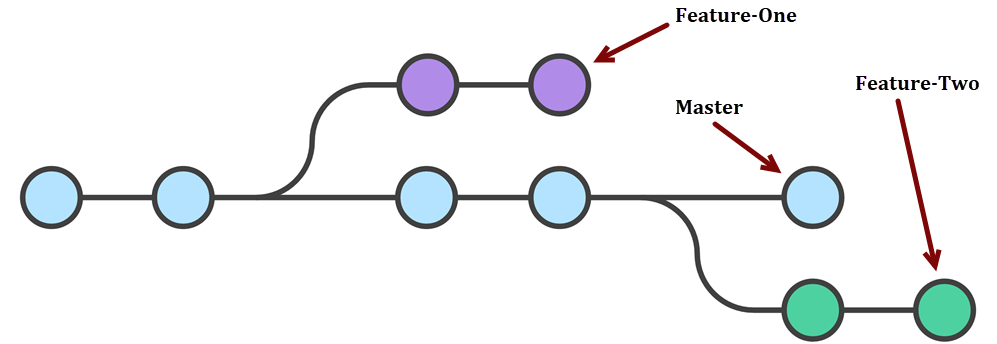
\includegraphics[width=\textwidth]{vcs-history}
\end{center}

\end{frame}


% \begin{frame}[fragile]{Version Control: merge - fast forward}
%
% \begin{center}
% 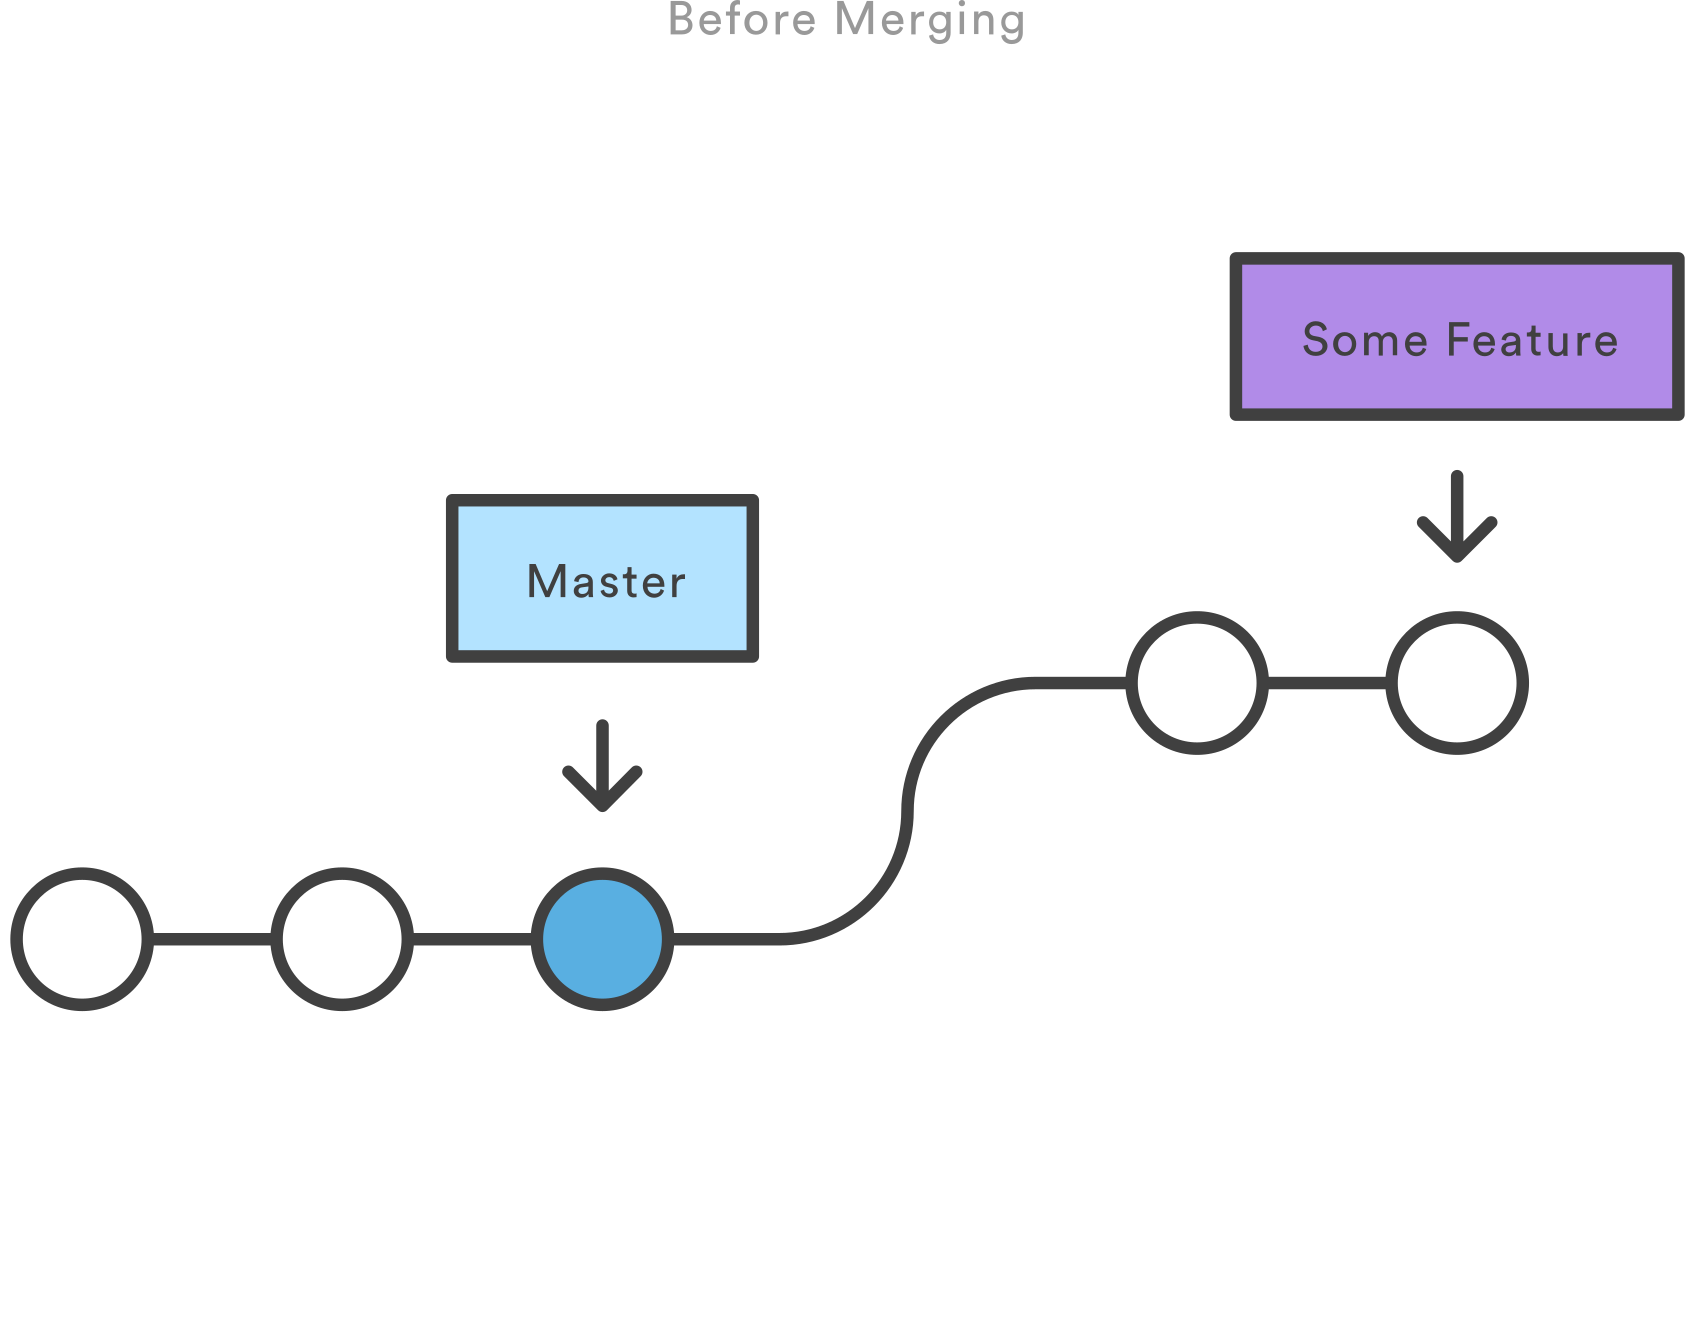
\includegraphics[width=\textwidth]{git-merge-ff}
% \end{center}
%
% \end{frame}
%
%
% \begin{frame}[fragile]{Version Control: - fast forward}
%
% \begin{center}
% 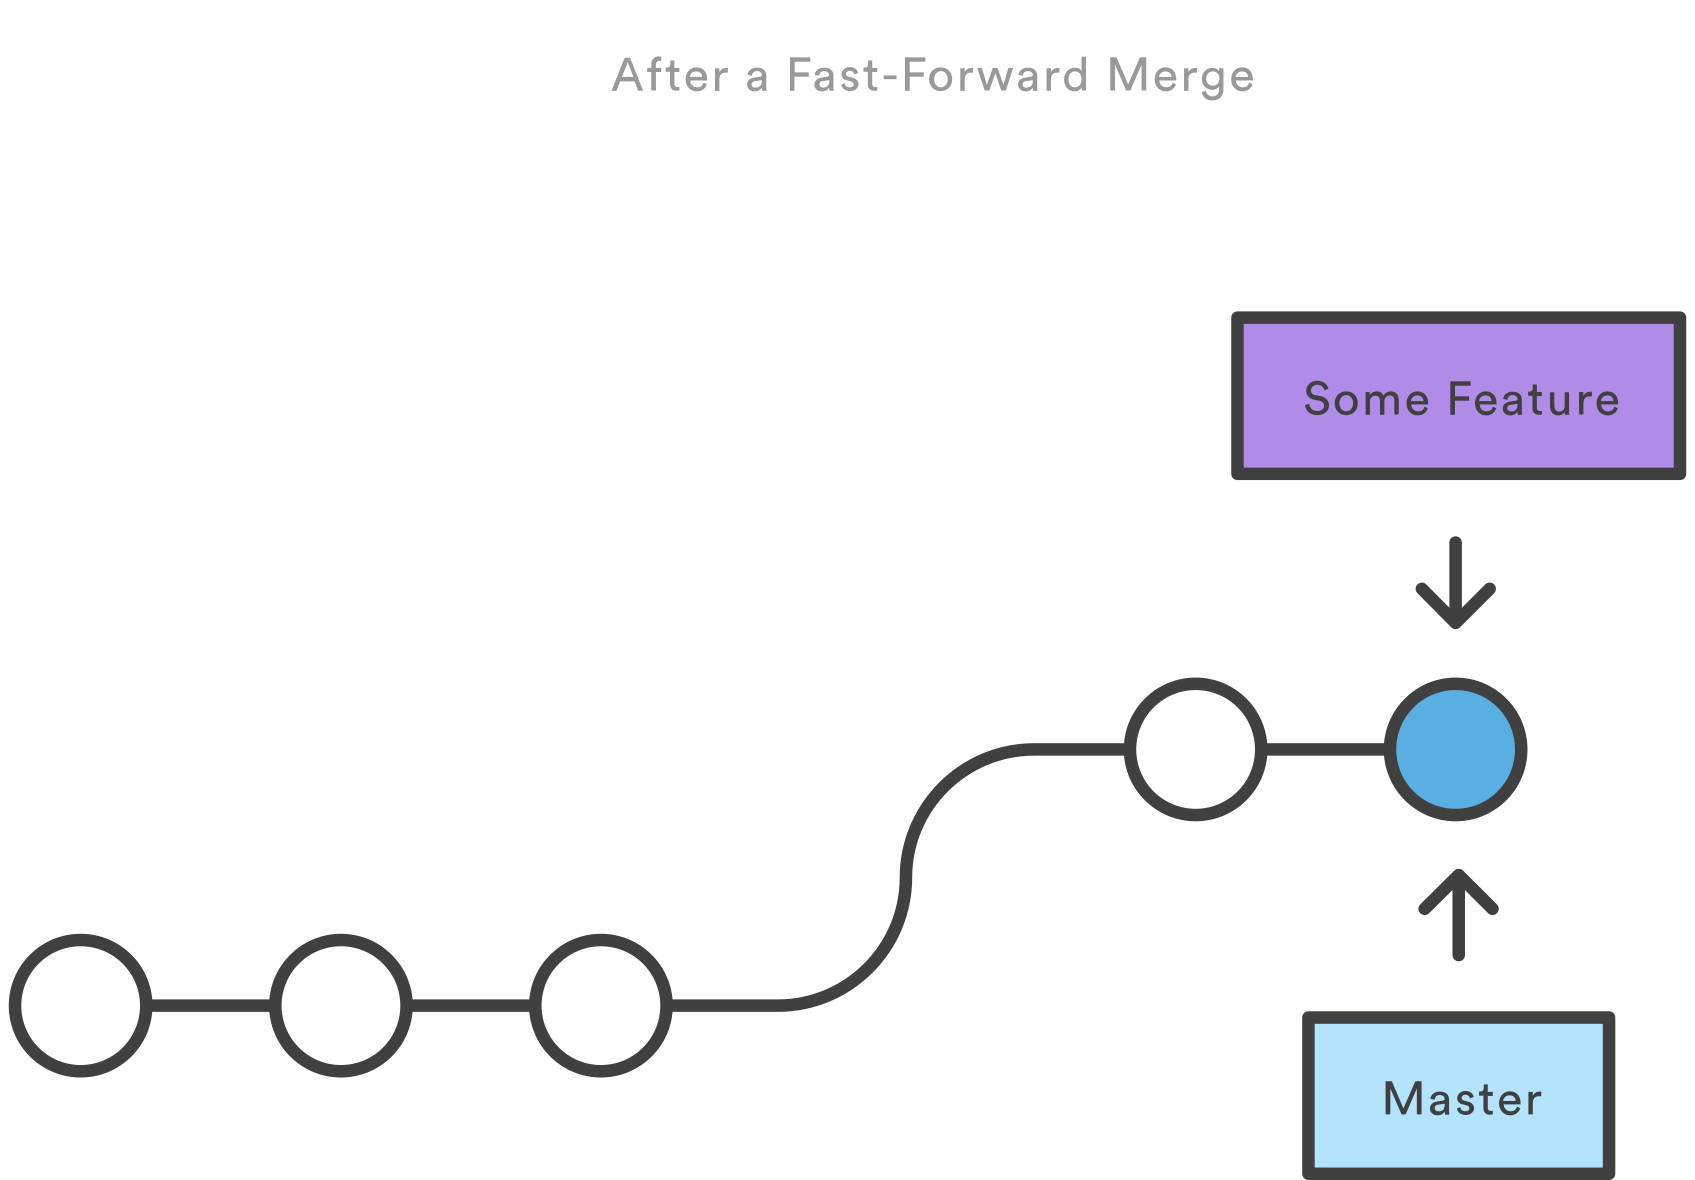
\includegraphics[width=\textwidth]{git-merge-ff2}
% \end{center}
%
% \end{frame}


\begin{frame}[fragile]{Version Control: merge - classic}

\begin{center}
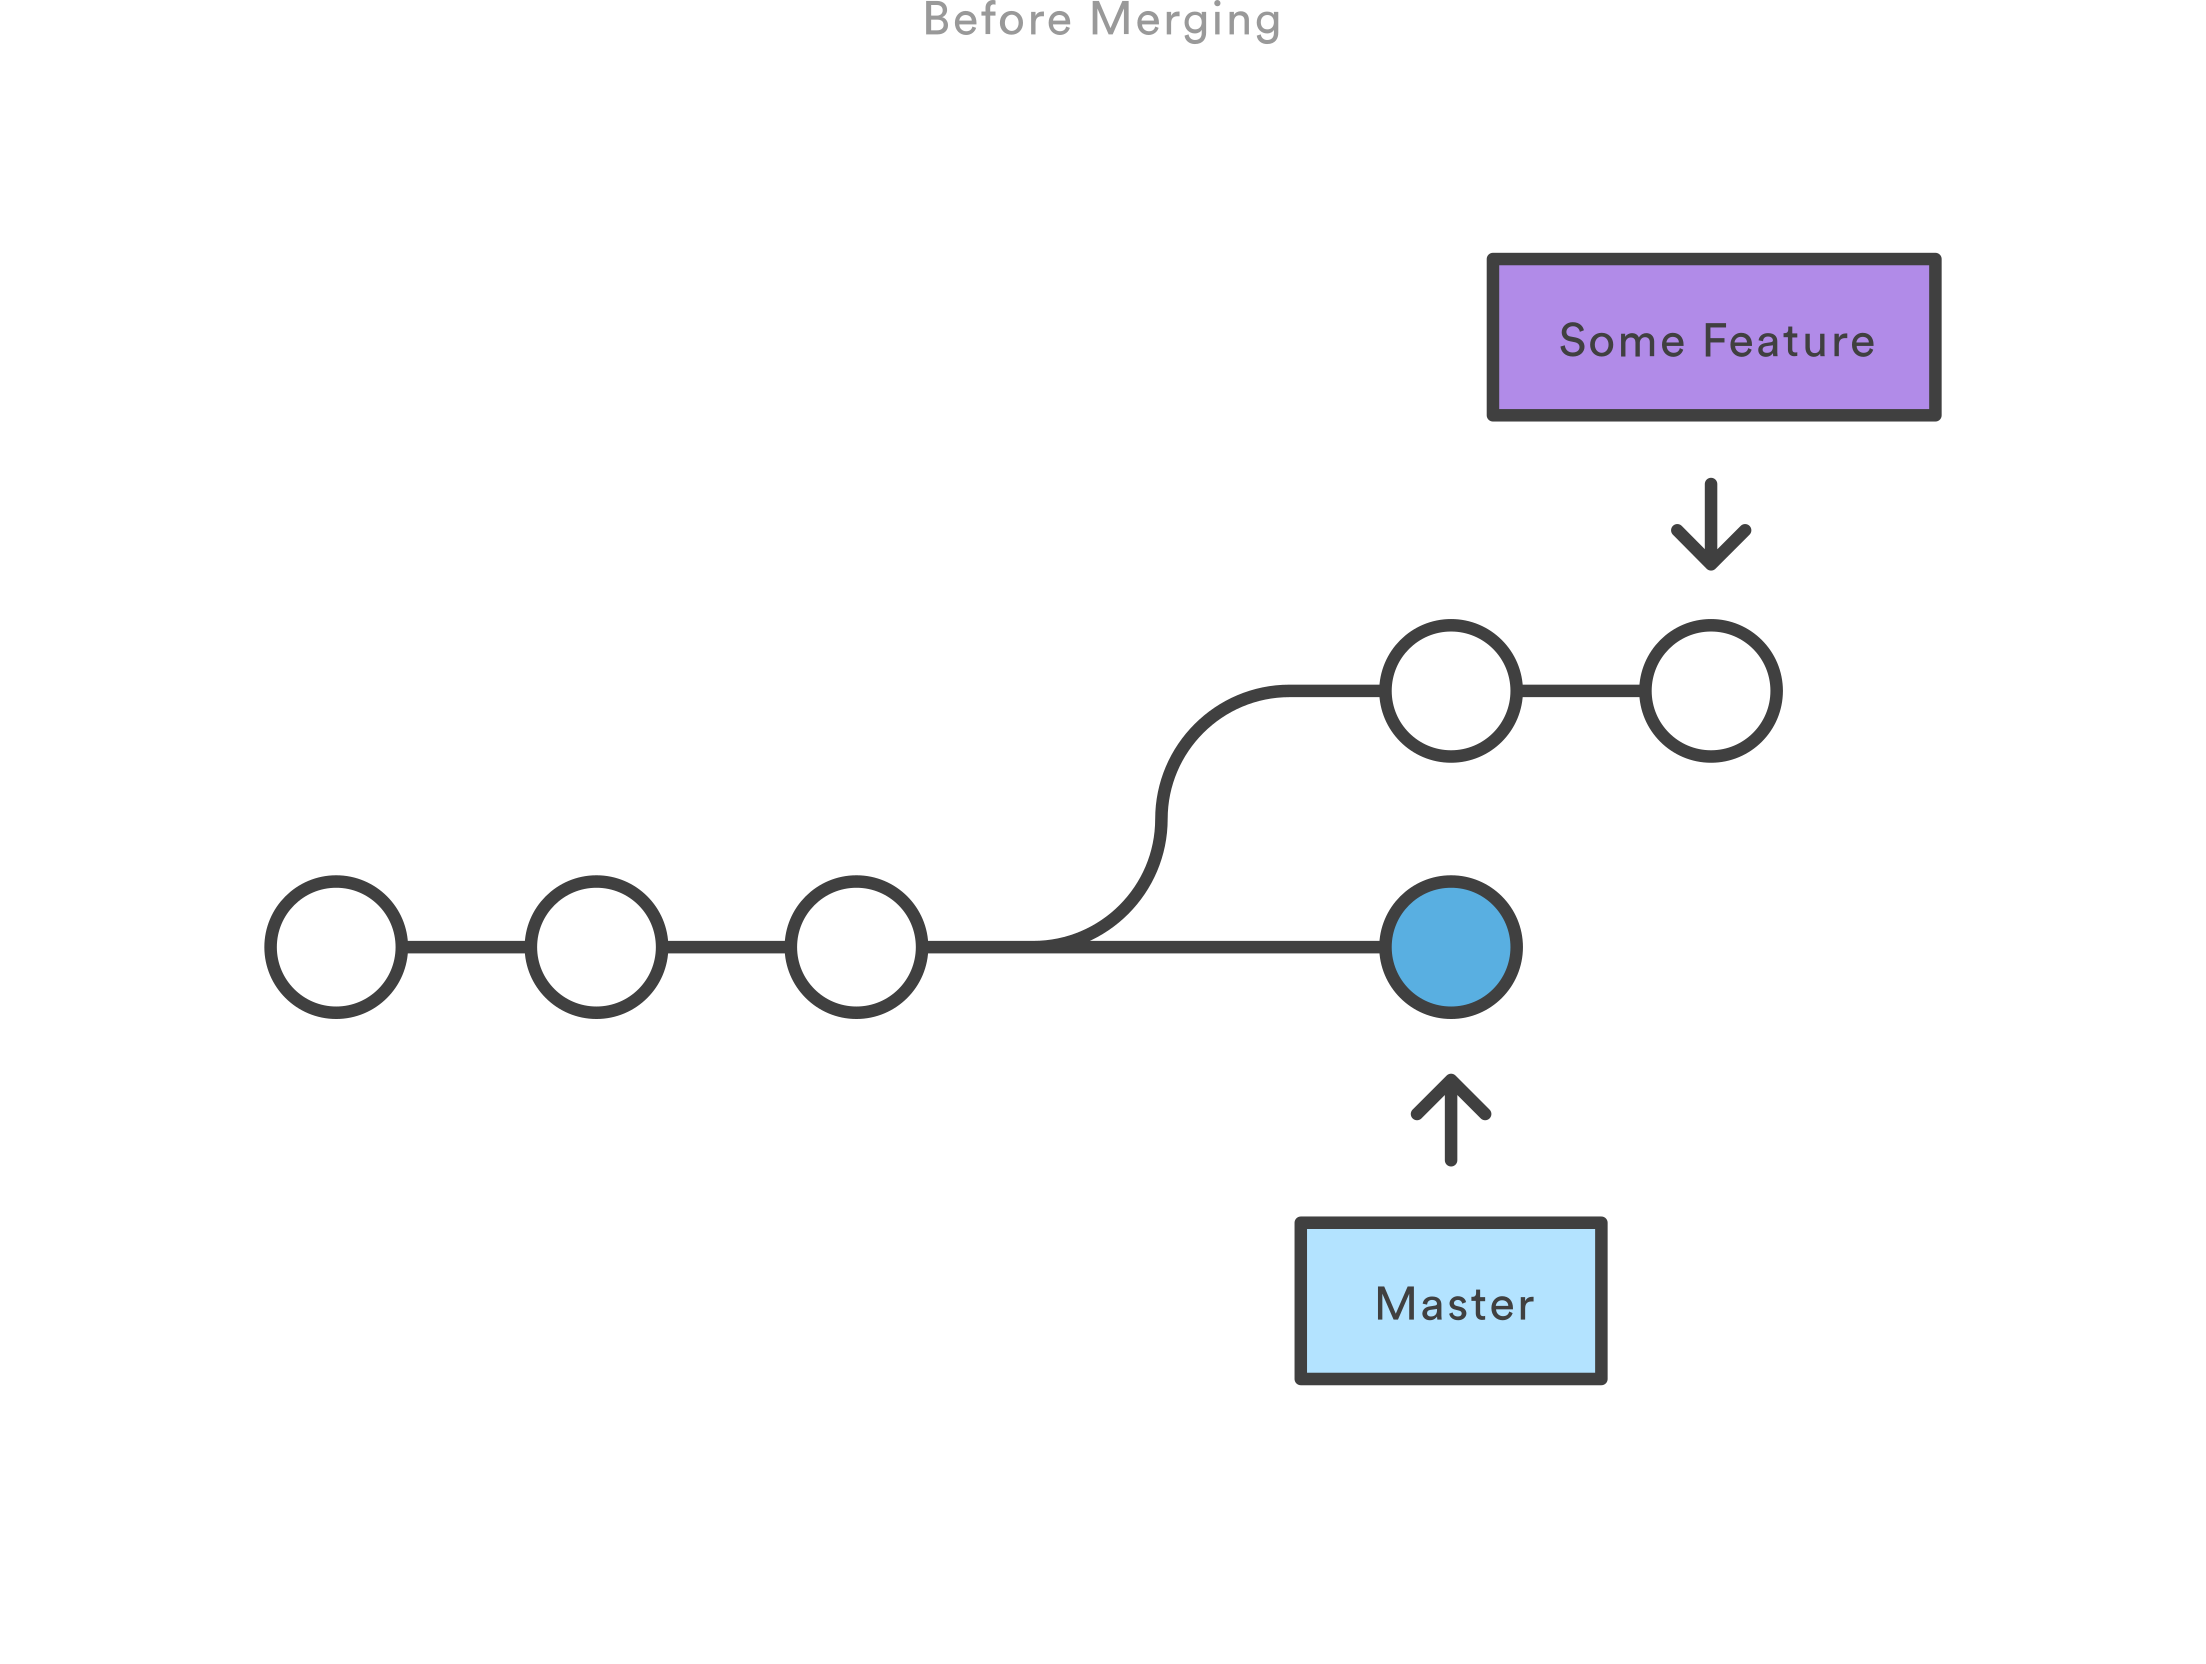
\includegraphics[width=\textwidth]{git-merge-nff}
\end{center}

\end{frame}

\begin{frame}[fragile]{Version Control: merge - classic}

\begin{center}
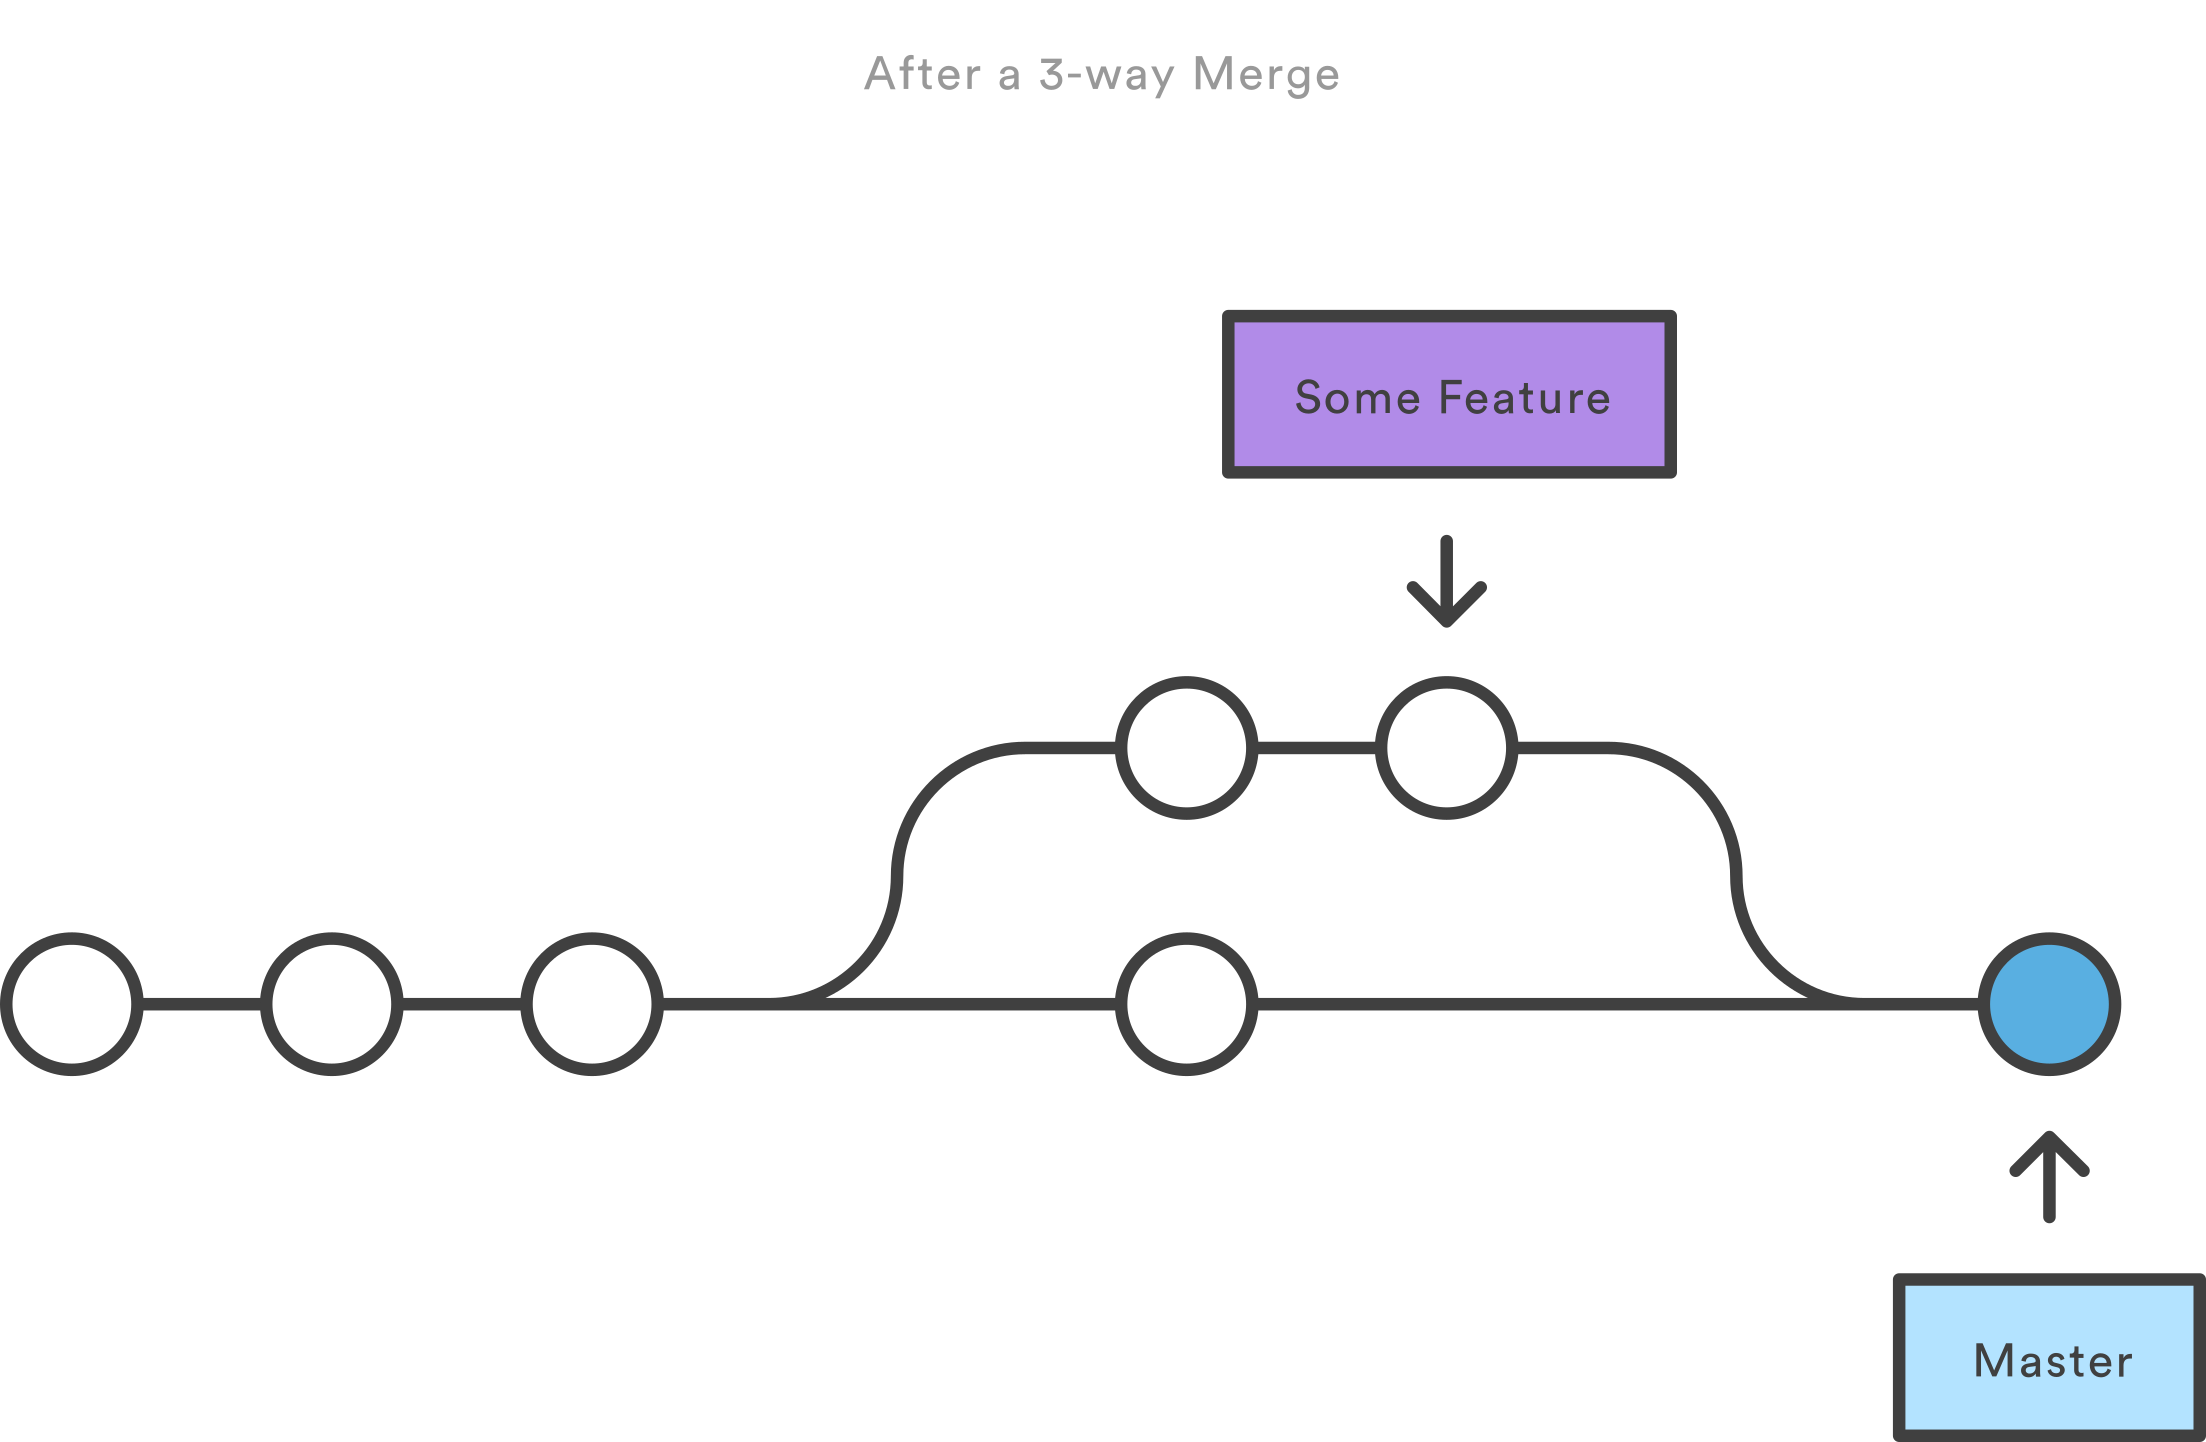
\includegraphics[width=\textwidth]{git-merge-nff2}
\end{center}

\end{frame}


\begin{frame}[fragile]{Traditional versus Distributed Version Control}

\begin{center}
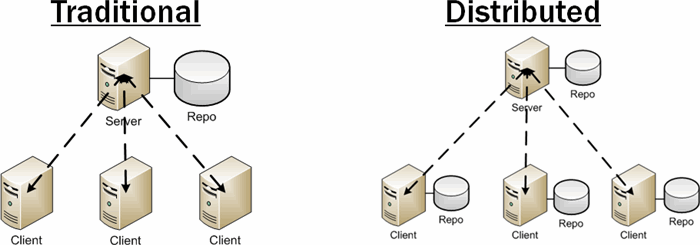
\includegraphics[width=0.7\textwidth]{vc-centralized-distributed}
\end{center}

\begin{columns}
\begin{column}{0.5\textwidth}
   \textbf{Traditional} (centralized)

   Everything lives in one place: the server. Easy to manage permissions,
     but it's not very flexible: single point of failure, clients needs to be
     constantly connected to the server, etc.
\end{column}
\begin{column}{0.5\textwidth}
  \textbf{Distributed}

  Each client has an entire copy of the repository. No single point of failure,
  no need of persistent links.
\end{column}
\end{columns}

\end{frame}




\begin{frame}[fragile]{Version control: hosting services}
\begin{itemize}
  \item Enables multiple git instances synchronization
  \item Provide ticketing systems (bugtracking/issue reporting system), project
  management, wiki for documentations
  \item Manage forks and pull requests
  \item ACL and fine granted access
\end{itemize}
\end{frame}


\begin{frame}[fragile]{Version control: well-known hosting services}


\begin{columns}
\begin{column}{0.5\textwidth}
  \begin{center}
  
\includegraphics[width=10em]{github-logo}

  
\includegraphics[width=5em]{gitlab-logo}

  
\includegraphics[width=10em]{bitbucket-logo}
  \end{center}
\end{column}
\begin{column}{0.5\textwidth}
  \begin{itemize}
    \item Most used public/private repository hosting platforms
    \item Many open source software are hosted in these services
    \item Mainly zero-cost for Open Source / Free Software, paid plans for private repositories
    \item Wiki, issues, pull requests
    \item Integrated Continuous integration and Continuous delivery
  \end{itemize}
\end{column}
\end{columns}

\end{frame}
